\section{Research Question}
\subsection{Motivation}
When you are working with databases, you will likely come in contact with the debate which is the most effective type of database management systems in terms of storing and managing the data. There are two main types: relational database management systems and non-relational database management systems. The choice of database management system can significantly impact the performance of a web application. Therefore, our project's focus is on investigating the effectiveness and performance of various database querying methods.

\subsection{Formulation}
Are there measurable and noticeable differences in different methods of searching through the coupons attributes inside the database, management system and what method performs the best? In terms of response times, is a relational or a non-relational database management system the best option? 

\subsection{Approach}
To answer our research question, we will be using the Python-based web framework Django and the Google Cloud Platform. The application will allow users to upload a coupon, write comments under coupons, create hashtags, up and down vote a coupon and see the score of the related coupon (see figure \ref{fig:useCaseCouponApp}). One main aspect of the application should be the search of a specific coupon based on for example a hashtag. We will implement both, a relational and non-relational database management system to store the coupon data and compare their performance in terms of response times for each search method.

\begin{figure}[h]
    \centering
    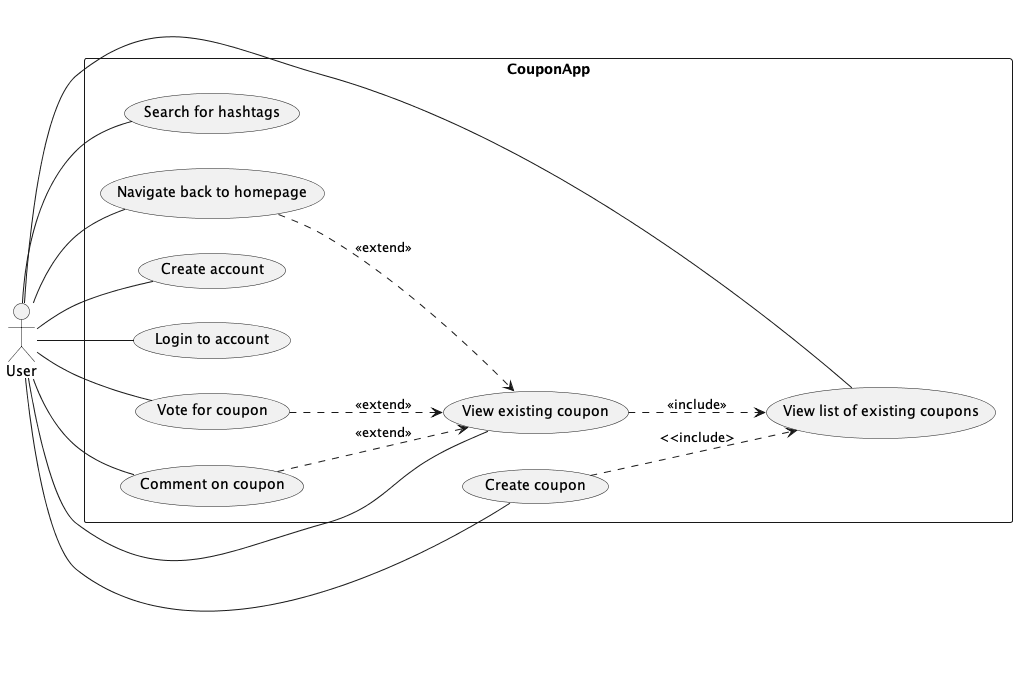
\includegraphics[scale=0.25]{resources/use_case.png}
    \caption{UML Use Case diagram - Coupon App}
    \label{fig:useCaseCouponApp}
\end{figure}

To collect the data on the performance of the different search methods, we will use a performance testing tool like "Google Cloud Load Testing". With tools like this, we are able to simulate many users accessing the coupon web application and measure the response times for different search queries. After we have collected the data, we will compare the mean response times and standard deviations for each search method and database management system and determine if there are significant differences in performance.

Our general approach is to develop a prototype coupon web application, test its performance using performance testing tools, and analyze the data collected from these tests to identify the most effective search methods and database management systems. By doing so, we aim to provide valuable insights for businesses looking to optimize their coupon web applications and improve the user experience for their customers.